\section{Resultado dos Cenários de Teste}

Após a apuração dos cenários descritos acima, chegamos aos seguintes resultados por serviço:

\begin{table}[H]
	\center
	\footnotesize
	\caption{Avaliação do serviço 2ª via de Conta }
	\label{tabela:avaliacaoSegundaViaConta}
	\begin{tabular}{|p{3cm}|p{3cm}|p{3cm}|}
		\hline
		\multicolumn{3}{|c|}{\textbf{2ª via de Conta}} \\
		\hline
		\textbf{Cenários}  	& \textbf{Situação} & \textbf{Percentual (\%)}  \\
		\hline		
		Cenário 1			& SUCESSO 		& (+) 33,33\% 	\\
		\hline
		Cenário 2 			& SUCESSO		& (+) 33,33\% 	\\
		\hline
		Cenário 3 			& FALHA 		& (+) 33,33\%	\\
		\hline		
		\multicolumn{2}{|c|}{\textbf{TOTAL}}	& 66\% 	\\
		\hline				
	\end{tabular}
	\legend{\fontsize{10}{12}\selectfont {Fonte: Autoria Própria}.}
\end{table}

O serviço de obter 2ª via de conta obteve o percentual de 66\% de sucesso nos cenários de testes aplicados sobre o produto gerado, conforme demostra a tabela \ref{tabela:avaliacaoSegundaViaConta}. 


\begin{table}[H]
	\center
	\footnotesize
	\caption{Informar Falta de Água}
	\label{tabela:avaliacaoInformarFaltaAgua}
	\begin{tabular}{|p{3cm}|p{3cm}|p{3cm}|}
		\hline
		\multicolumn{3}{|c|}{\textbf{Informar Falta de Água}} \\
		\hline
		\textbf{Cenários}  	& \textbf{Situação} & \textbf{Percentual (\%)}  \\
		\hline		
		Cenário 1			& SUCESSO 		& (+) 33,33\% 	\\
		\hline
		Cenário 2 			& SUCESSO		& (+) 33,33\% 	\\
		\hline
		Cenário 3 			& SUCESSO 		& (+) 33,33\%	\\
		\hline		
		\multicolumn{2}{|c|}{\textbf{TOTAL}}	& 100\% 	\\
		\hline				
	\end{tabular}
	\legend{\fontsize{10}{12}\selectfont {Fonte: Autoria Própria}.}
\end{table}

O serviço de Informar Falta de Água obteve o percentual de 100\% de sucesso nos cenários de testes aplicados sobre o produto gerado, conforme demostra a tabela \ref{tabela:avaliacaoInformarFaltaAgua}.


\begin{table}[H]
	\center
	\footnotesize
	\caption{Solicitar Restabelecimento da Ligação}
	\label{tabela:avaliacaoRestabelerLigacaoAgua}
	\begin{tabular}{|p{3cm}|p{3cm}|p{3cm}|}
		\hline
		\multicolumn{3}{|c|}{\textbf{Solicitar Restabelecimento da Ligação}} \\
		\hline
		\textbf{Cenários}  	& \textbf{Situação} & \textbf{Percentual (\%)}  \\
		\hline		
		Cenário 1			& SUCESSO 		& (+) 33,33\% 	\\
		\hline
		Cenário 2 			& SUCESSO		& (+) 33,33\% 	\\
		\hline
		Cenário 3 			& SUCESSO 		& (+) 33,33\%	\\
		\hline		
		\multicolumn{2}{|c|}{\textbf{TOTAL}}	& 100\% 	\\
		\hline				
	\end{tabular}
	\legend{\fontsize{10}{12}\selectfont {Fonte: Autoria Própria}.}
\end{table}

O serviço de Solicitar Restabelecimento da Ligação obteve o percentual de 100\% de sucesso nos cenários de testes aplicados sobre o produto gerado, conforme demostra a tabela \ref{tabela:avaliacaoRestabelerLigacaoAgua}.



\section{Apresentação dos Resultados Obtidos}

Levando em consideração os resultados obtidos através da aplicação de todos os cenários de testes descritos acima sob os serviços desenvolvidos neste trabalho,
é possível afirmar que a utilização da uma URA para realizar o atendimento de primeiro nível tem potencial para reduzir parte dos atendimentos destinados à solicitação de 2ª via de conta, falta de água e restabelecimento da ligação, definindo na padronização dos atendimentos e contribuindo para a redução dos custos.
 
 %observando os percentuais atingidos com base na média descrita dos principais %Serviços do Atendimento ao Público, notamos que a solução proposta é capaz de %reduzir em até 20,46\%, dos registros de atendimentos diários, conforme visto %abaixo na figura \ref{figura:eficienciaServicos}:	

%\begin{figure}[!htb]
%	\centering
%	\caption{Gráfico de avaliação dos serviços automatizados}
%	\label{figura:eficienciaServicos}	
%	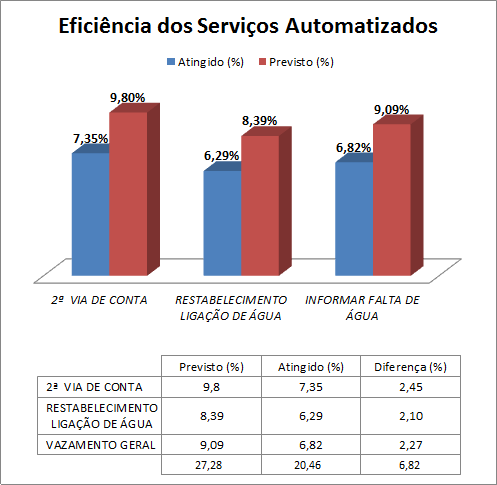
\includegraphics{figuras/eficiencia_servicos.png}
%	\legend {\fontsize{10}{12}\selectfont {Fonte: Autoria Própria}.}
%\end{figure}

